\documentclass[11pt,a4paper,final]{article} %draft

\usepackage[T1,T2A]{fontenc}
\usepackage[utf8]{inputenc}
\usepackage[english, russian]{babel}

\usepackage[final]{pdfpages}

\usepackage{textcomp,enumitem}

\usepackage{amsmath,amsthm,amssymb}

\usepackage{fancyhdr} % для настройки страницы и колонтитулов

\usepackage{graphicx}

\usepackage{indentfirst} % автоматический отступ в начале каждого раздела

\usepackage[unicode, pdftex, colorlinks, urlcolor=blue]{hyperref}

\usepackage[left=2cm,right=2cm,top=2cm,bottom=2cm,bindingo ffset=0cm]{geometry}

\linespread{1.3} % устанавливает междустрочный интервал

\pagestyle{plain} % для отображения номеров внизу 

\usepackage{float}

\usepackage{listings} 

\usepackage{pdflscape}
\usepackage{listings} 
\definecolor{darkgreen}{rgb}{0,0.5,0}
\usepackage{subcaption}


\lstset{
	backgroundcolor=\color{white},  % Устанавливаем белый фон для блока кода
	basicstyle=\ttfamily\small\fontfamily{inconsolata}\selectfont,  % Основной стиль текста: моноширинный шрифт Inconsolata с небольшим размером
	commentstyle=\color{darkgreen}\slshape,  % Комментарии будут зелеными и курсивными
	keywordstyle=\color{blue}\bfseries,  % Ключевые слова выделяются синим цветом и полужирным шрифтом
	numberstyle=\scriptsize\color{gray},  % Стиль нумерации строк: маленький размер шрифта и серый цвет
	stringstyle=\color{orange},  % Строки (текст в кавычках) отображаются оранжевым цветом
	breakatwhitespace=false,  % Не прерывать строки только по пробелам
	breaklines=true,  % Автоматический перенос длинных строк
	postbreak=\mbox{\textcolor{gray}{$\hookrightarrow$}}, % Символ переноса строки
	captionpos=b,  % Позиция заголовка/описания для блока кода — внизу (b — bottom)
	keepspaces=true,  % Сохранить пробелы, как они есть, в исходном коде
	numbers=left,  % Нумерация строк будет отображаться слева
	numbersep=5pt,  % Отступ между строками кода и номерами строк (4pt)
	showspaces=false,  % Не показывать пробелы
	showstringspaces=false,  % Не показывать пробелы внутри строк
	showtabs=false,  % Не показывать символы табуляции
	tabsize=4,  % Размер табуляции — 4 пробела
	language=Haskell,  % Указываем язык программирования для синтаксического подсветки (C++)
	captionpos=t,  % Заголовок кода будет размещен вверху (t — top)
	xleftmargin=0mm,  % Убираем отступ слева
	frame=single,  % Однотонная рамка вокруг блока кода
	framerule=0.25mm,  % Толщина рамки — 0.25 мм
	literate=
	{а}{{\selectfont\char224}}1
	{б}{{\selectfont\char225}}1
	{в}{{\selectfont\char226}}1
	{г}{{\selectfont\char227}}1
	{д}{{\selectfont\char228}}1
	{е}{{\selectfont\char229}}1
	{ж}{{\selectfont\char230}}1
	{з}{{\selectfont\char231}}1
	{и}{{\selectfont\char232}}1
	{й}{{\selectfont\char233}}1
	{к}{{\selectfont\char234}}1
	{л}{{\selectfont\char235}}1
	{м}{{\selectfont\char236}}1
	{н}{{\selectfont\char237}}1
	{о}{{\selectfont\char238}}1
	{п}{{\selectfont\char239}}1
	{р}{{\selectfont\char240}}1
	{с}{{\selectfont\char241}}1
	{т}{{\selectfont\char242}}1
	{у}{{\selectfont\char243}}1
	{ф}{{\selectfont\char244}}1
	{х}{{\selectfont\char245}}1
	{ц}{{\selectfont\char246}}1
	{ч}{{\selectfont\char247}}1
	{ш}{{\selectfont\char248}}1
	{щ}{{\selectfont\char249}}1
	{ъ}{{\selectfont\char250}}1
	{ы}{{\selectfont\char251}}1
	{ь}{{\selectfont\char252}}1
	{э}{{\selectfont\char253}}1
	{ю}{{\selectfont\char254}}1
	{я}{{\selectfont\char255}}1
	{А}{{\selectfont\char192}}1
	{Б}{{\selectfont\char193}}1
	{В}{{\selectfont\char194}}1
	{Г}{{\selectfont\char195}}1
	{Д}{{\selectfont\char196}}1
	{Е}{{\selectfont\char197}}1
	{Ж}{{\selectfont\char198}}1
	{З}{{\selectfont\char199}}1
	{И}{{\selectfont\char200}}1
	{Й}{{\selectfont\char201}}1
	{К}{{\selectfont\char202}}1
	{Л}{{\selectfont\char203}}1
	{М}{{\selectfont\char204}}1
	{Н}{{\selectfont\char205}}1
	{О}{{\selectfont\char206}}1
	{П}{{\selectfont\char207}}1
	{Р}{{\selectfont\char208}}1
	{С}{{\selectfont\char209}}1
	{Т}{{\selectfont\char210}}1
	{У}{{\selectfont\char211}}1
	{Ф}{{\selectfont\char212}}1
	{Х}{{\selectfont\char213}}1
	{Ц}{{\selectfont\char214}}1
	{Ч}{{\selectfont\char215}}1
	{Ш}{{\selectfont\char216}}1
	{Щ}{{\selectfont\char217}}1
	{Ъ}{{\selectfont\char218}}1
	{Ы}{{\selectfont\char219}}1
	{Ь}{{\selectfont\char220}}1
	{Э}{{\selectfont\char221}}1
	{Ю}{{\selectfont\char222}}1
	{Я}{{\selectfont\char223}}1,
	numbers=left, % пронумеровать строки с левой стороны
	breaklines=true % разрешает автоматический перенос строк
}

\hypersetup{
	colorlinks=true, % делает ссылки цветными вместо рамки
	linkcolor=blue, % цвет внутренних ссылок
	urlcolor=blue, % цвет внешних ссылок
	citecolor=blue % цвет ссылок на литературу в тексте
}

\textheight=24cm 
\textwidth=16cm
\oddsidemargin=0pt 
\topmargin=-1.5cm
\parindent=24pt 
\parskip=0pt 
\tolerance=2000 
\flushbottom 

%\usepackage[font=scriptsize]{caption}
\usepackage[labelsep=period]{caption}

\usepackage{amsmath}
\usepackage{multirow} 
\usepackage{tabularx}

\newcommand{\specialcell}[2][l]{\begin{tabular}[#1]{@{}l@{}}#2\end{tabular}}

\begin{document}
	
\thispagestyle{empty}

\begin{center}
	{\Large МИНОБРНАУКИ РОССИИ}\\
	~\\
	{\large ФЕДЕРАЛЬНОЕ ГОСУДАРСТВЕННОЕ БЮДЖЕТНОЕ ОБРАЗОВАТЕЛЬНОЕ УЧРЕЖДЕНИЕ ВЫСШЕГО ПРОФЕССИОНАЛЬНОГО ОБРАЗОВАНИЯ}\\
	~\\
	{\Large \bf <<САНКТ-ПЕТЕРБУРГСКИЙ ПОЛИТЕХНИЧЕСКИЙ УНИВЕРСИТЕТ ПЕТРА ВЕЛИКОГО>>}\\
	~\\
	{\large Институт компьютерных наук и кибербезопасности }\\
	{\large Высшая школа технологий искусственного интеллекта}\\
	{\large Направление 02.03.01 Математика и компьютерные науки}\\
	~\\
	~\\
	~\\
	~\\
	{\Large \bf  Отчет по лабораторной работе №4 }\\
	\vspace{3mm}
	{\Large {по дисциплине <<Функциональное программирование>>}}\\
	\vspace{3mm}
	{\Large {Вариант 4}}\\
	~\\
	~\\
	~\\
	~\\
	~\\
	~\\
	{\large Обучающийся: \underline{\hspace{3.5cm}} \hspace{12mm} Шихалев А.О.}\\
	~\\
	{\large Руководитель: \underline{\hspace{3.5cm}} \hspace{12mm} Моторин Д.Е.}\\
	~\\
	~\\
	~\\
	~\\
	~\\
\end{center}
\begin{flushright}
	
	«\underline{\hspace{1cm}}»\underline{\hspace{3cm}}20\underline{\hspace{0.7cm}}г.
\end{flushright}
~\\
~\\
\begin{center}
	{\large Санкт-Петербург, 2024}
\end{center}

\newpage

\tableofcontents

\newpage
\section*{Введение}
\addcontentsline{toc}{section}{Введение}
Практическое задание №4 представляет собой реализацию следующего заданий: 

\begin{enumerate}

	\item \textbf{Функция 1:} Написать функцию сложения по модулю addMod :: Int -> Int -> Int -> Int, которая принимает три целых числа: два слагаемых и модуль и возвращает сумму двух чисел по модулю. Используя QuickCheck, проверить следующие свойства:
	\begin{enumerate}
		\item Сложение по модулю: (addMod x y m) mod m == (x + y) mod m.
		\item Нейтральный элемент: addMod x 0 m == x mod m.
		\item Коммутативность: addMod x y m == addMod y x m.
	\end{enumerate}
	
	\item \textbf{Функция 2:} Реализовать функцию treeDepth :: Tree a -> Int, где Tree a -- бинарное дерево, определяемое как: data Tree a = Empty | Node a (Tree a)(Tree a). Используя QuickChech, проверить следующие свойства:
	
	\begin{enumerate}
		\item Глубина пустого дерева равна 0.
		\item Глубина дерева с одним узлом равна 1.
		\item Глубина дерева с двумя ветвями равна максимальной глубине среди ветвей плюс 1.
		\item Добавление узла в дерево не уменьшает его глубину.
	\end{enumerate}
\end{enumerate}

\par Лабораторная работа выполнена на языке Haskell в текстовом редакторе Visual Studio Code 1.95.3.


\newpage
\section {Математическое описание}

\textbf{QuickCheck} — это инструмент для автоматической проверки свойств программ. Он использует метод генерации тестов с последующей проверкой утверждений о программе с использованием случайных данных. QuickCheck позволяет описывать свойства функций в виде логических выражений, и затем автоматически проверять их с помощью случайных значений. 

В Haskell для работы с QuickCheck есть несколько основных команд и функций, которые позволяют генерировать тесты и проверять свойства:

\begin{itemize}
	\item \textbf{ quickCheck:} Команда для запуска проверки свойства. Она принимает функцию с описанием свойства и автоматически генерирует случайные входные данные для тестирования.
	\item\textbf{ Property:} Это тип, который представляет собой проверку логического свойства, которое может быть либо истинным, либо ложным, в зависимости от входных данных. Он часто используется с операторами, такими как ==>, чтобы описать свойства, которые должны выполняться при определённых условиях.
\end{itemize}

Для того чтобы QuickCheck мог генерировать случайные данные для тестов, необходимо определить, как создавать случайные значения для тех типов данных, которые используются в тестируемых функциях. Это делается через класс Arbitrary.
\par \textbf{Arbitrary} — это класс типов, который предоставляет метод arbitrary, используемый для генерации случайных значений. Для каждого типа, для которого мы хотим генерировать случайные значения, нужно предоставить инстанс этого класса.

\newpage
\section{Особенности реализации}

\subsection{Функция 1}

\textbf{addMod} — это функция, которая выполняет сложение двух целых чисел по модулю третьего числа. Формально, она вычисляет сумму двух чисел $x$ и $y$, а затем результат делится по модулю $z$. То есть функция возвращает остаток от деления суммы чисел $x$ и $y$ на число $z$. Функция представлена на листинге \ref{lst:l1}.

\begin{lstlisting}[caption={Функция вычисления суммы двух чисел по модулю третьего числа}, label={lst:l1}]
addMod :: Int -> Int -> Int -> Int
addMod x y z = (x + y) `mod` z
\end{lstlisting}

где: $x, y, z$ — целые числа ($\text{Int}$), операция $\mod$ возвращает остаток от деления $(x + y)$ на $z$.

Далее были написаны тесты для проверки следующих свойств:
\begin{enumerate}
\item \textbf{Сложение по модулю:} (addMod x y m) mod m == (x + y) mod m.

\begin{lstlisting}[caption={Код теста №1}, label={lst:l2}]
prop_mod :: Int -> Int -> Int -> Property
prop_mod x y m = (m /= 0) ==> (addMod x y m) `mod` m === (x + y) `mod` m  
\end{lstlisting}

\item \textbf{ Нейтральный элемент:} addMod x 0 m == x mod m.
Функция представлена на листинге \ref{lst:l2}.

\begin{lstlisting}[caption={Код теста для нейтрального элемента}, label={lst:l2}]
prop_neutral :: Int -> Int -> Property
prop_neutral x m = (m /= 0) ==> addMod x 0 m === x `mod` m
\end{lstlisting}

\item \textbf{Коммутативность:} addMod x y m == addMod y x m.
Функция представлена на листинге \ref{lst:l3}.
\begin{lstlisting}[caption={Код теста для коммутативности}, label={lst:l3}]
prop_commutativity :: Int -> Int -> Int -> Property
prop_commutativity x y m = (m /= 0) ==> addMod x y m === addMod y x m
\end{lstlisting}
\end{enumerate}

\subsection{Функция 2}

\textbf{Tree} — это рекурсивный тип данных, представляющий бинарное дерево, где каждый узел может иметь два дочерних элемента, а также может быть пустым. Тип данных \texttt{Tree} объявляется следующим образом:

\begin{lstlisting}[caption={Объявление типа данных Tree}, label={lst:l1}]
data Tree a = Empty | Node a (Tree a) (Tree a) deriving Show
\end{lstlisting}

Функция \textbf{treeDepth} вычисляет глубину дерева. Глубина дерева определяется как максимальное количество узлов от корня до самого глубокого листа. Если дерево пустое (\texttt{Empty}), его глубина равна 0. Для узла глубина равна 1 плюс максимальная глубина его левого и правого поддеревьев.

\begin{lstlisting}[caption={Функция вычисления глубины дерева}, label={lst:l2}]
treeDepth :: Tree a -> Int
treeDepth Empty = 0
treeDepth (Node _ left right) = 1 + max (treeDepth left) (treeDepth right)
\end{lstlisting}

Далее были написаны тесты для проверки следующих свойств:
\begin{enumerate}
\item \textbf{Глубина пустого дерева:} Глубина пустого дерева должна быть равна 0. Тест представлен на листинге \ref{lst:l3}.

\begin{lstlisting}[caption={Тест для проверки глубины пустого дерева}, label={lst:l3}]
prop_emptyTree :: Bool
prop_emptyTree = treeDepth (Empty :: Tree Int) == 0
\end{lstlisting}

\item \textbf{Глубина дерева с одним узлом:} Глубина дерева с одним узлом должна быть равна 1. Тест представлен на листинге \ref{lst:l4}.

\begin{lstlisting}[caption={Тест для проверки глубины дерева с одним узлом}, label={lst:l4}]
prop_singleNodeTree :: Bool
prop_singleNodeTree = treeDepth (Node 1 Empty Empty :: Tree Int) == 1
\end{lstlisting}

\item \textbf{Глубина дерева с двумя ветвями:} Глубина дерева с двумя ветвями должна быть равна максимальной глубине среди ветвей плюс 1. Тест представлен на листинге \ref{lst:l5}.

\begin{lstlisting}[caption={Тест для проверки глубины дерева с двумя ветвями}, label={lst:l5}]
prop_twoBranchTree :: Tree Int -> Tree Int -> Bool
prop_twoBranchTree leftBranch rightBranch =
let tree = Node 1 leftBranch rightBranch
in treeDepth tree == 1 + max (treeDepth leftBranch) (treeDepth rightBranch)
\end{lstlisting}

\item \textbf{Добавление узла в дерево не уменьшает его глубину:} При добавлении узла в дерево его глубина не уменьшается. Тест представлен на листинге \ref{lst:l6}.

\begin{lstlisting}[caption={Тест для проверки добавления узла в дерево}, label={lst:l6}]
prop_addNodeInTree :: Tree Int -> Int -> Bool
prop_addNodeInTree tree x =
let newTree = Node x tree Empty
in treeDepth newTree >= treeDepth tree
\end{lstlisting}
\end{enumerate}


\subsection{Генерация случайных данных с помощью Arbitrary}

В Haskell библиотека QuickCheck предоставляет тип \texttt{Arbitrary}, который используется для автоматической генерации случайных значений для тестируемых типов. Чтобы использовать QuickCheck для тестирования типов данных, необходимо определить экземпляр типа \texttt{Arbitrary} для этого типа данных. В случае с деревьями мы определили экземпляр \texttt{Arbitrary} для типа данных \texttt{Tree a}, который позволяет QuickCheck генерировать случайные деревья для тестирования.

Тип данных \texttt{Arbitrary} выглядит следующим образом:

\begin{lstlisting}[caption={Интерфейс типа Arbitrary}, label={lst:l7}]
class Arbitrary a where
arbitrary :: Gen a
\end{lstlisting}

Функция \texttt{arbitrary} генерирует случайные значения для типа \texttt{a}, и в случае с деревьями мы определяем, как генерировать случайные деревья. В нашем примере используется функция \texttt{sized}, которая позволяет задать ограничение на глубину генерируемого дерева.

Вот как выглядит реализация \texttt{Arbitrary} для типа \texttt{Tree}:

\begin{lstlisting}[caption={Определение Arbitrary для типа Tree}, label={lst:l8}]
instance Arbitrary a => Arbitrary (Tree a) where
arbitrary = sized genTree
where
genTree 0 = return Empty
genTree n = frequency
[ (1, return Empty)
, (5, Node <$> arbitrary <*> genTree (n-1) <*> genTree (n-1))
]
\end{lstlisting}

Здесь:
- \texttt{sized} позволяет задавать глубину дерева, передавая параметр глубины в функцию \texttt{genTree}.
- Когда глубина дерева равна 0 (\texttt{genTree 0}), генерируется пустое дерево (\texttt{Empty}).
- Для большей глубины (\texttt{genTree n}) с использованием \texttt{frequency} выбираются варианты: с вероятностью 1 генерируется пустое дерево, с вероятностью 5 создается узел дерева с рекурсивно генерируемыми поддеревьями.

\subsection{Функция main}
Функция \texttt{main} является точкой входа программы, в которой выполняются тесты для проверки свойств различных функций. В частности, для каждого теста используется функция \texttt{quickCheck}, которая автоматически проверяет заданное свойство на случайных данных.

Функция представлена на листинге \ref{lst:l9}.

\begin{lstlisting}[caption={Код функции main}, label={lst:l9}]
main :: IO()
main = do 
putStrLn "Сложение по модулю: "
quickCheck prop_mod
putStrLn "Нейтральный элемент: "
quickCheck prop_neutral
putStrLn "Коммутативность: "
quickCheck prop_commutativity
putStrLn "\nГлубина пустого дерева равна 0: "
quickCheck prop_emptyTree
putStrLn "Глубина дерева с одним узлом равна 1: "
quickCheck prop_singleNodeTree 
putStrLn "Глубина дерева с двумя ветвями равна максимальной глубине среди ветвей плюс 1: "
quickCheckWith stdArgs { maxSuccess = 100, maxSize = 10 } prop_twoBranchTree
putStrLn "Добавление узла в дерево не уменьшает его глубину: "
quickCheckWith stdArgs { maxSuccess = 100, maxSize = 10 } prop_addNodeInTree
\end{lstlisting}

\newpage
\section{Результаты работы программы}
Результаты запуска программы с помощью команды \texttt{stack test} представлены на рисунке \ref{fig:res}

\begin{figure}[h]
	\centering
	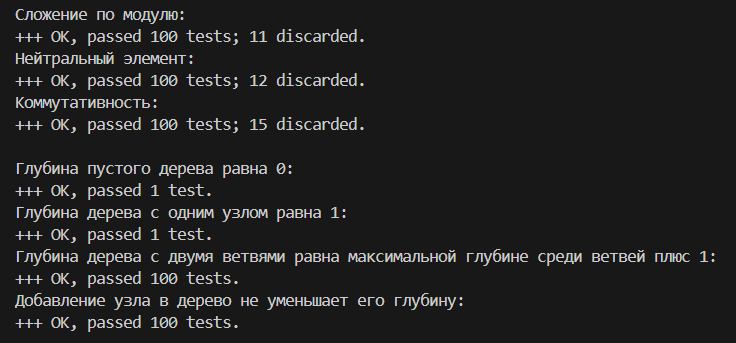
\includegraphics[width=0.7\linewidth]{img/res.png}
	\caption{Результаты работы программы в консоли.}
	\label{fig:res}
\end{figure}
	
Тестирование каждого свойства функций \texttt{addMod} и \texttt{treeDepth} с использованием QuickCheck на наборе 100 случайных входных данных было успешно завершено, все тесты пройдены.

В случае, если функция будет некорретно вычислять значение, тесты свойств будут провалены, как показано на \hyperref[fig:f1]{рисунке 2.} 

\begin{figure}[h]
	\centering
	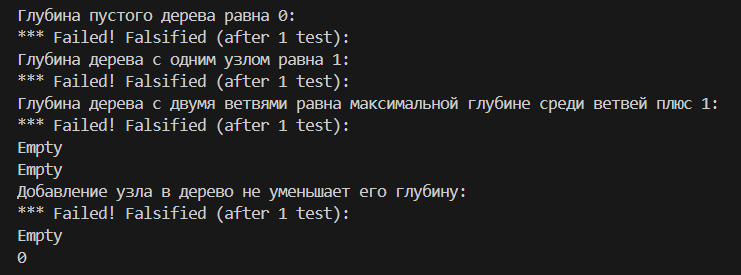
\includegraphics[width=0.75\linewidth]{img/f1.png}
	\caption{Тесты провалены.}
	\label{fig:f1}
\end{figure}

Для этого мы изменили функцию \texttt{treeDepth}, код измененной функции представлен в \hyperref[lst:l10]{листинге 14.} 

\begin{lstlisting}[caption={Код измененной функции treeDepth}, label={lst:l10}]
treeDepth :: Tree a -> Int
treeDepth Empty = -1
treeDepth (Node _ left right) = -5 + max (treeDepth left) (treeDepth right)
\end{lstlisting}



\newpage
\section*{Заключение}
\addcontentsline{toc}{section}{Заключение}

В ходе выполнения лабораторной работы была реализована и протестирована на корректность несколько функций в языке программирования Haskell. В частности, была реализована функция сложения по модулю, которая принимает три целых числа и возвращает остаток от деления суммы этих чисел на третье число. Для этой функции были написаны тесты с использованием библиотеки QuickCheck, проверяющие такие свойства, как сложение по модулю, нейтральный элемент и коммутативность операции.

Кроме того, была реализована функция для вычисления глубины бинарного дерева, представленного типом данных \texttt{Tree}. Для этой функции также были разработаны тесты с использованием QuickCheck, которые проверяют такие свойства, как глубина пустого дерева, глубина дерева с одним узлом, глубина дерева с двумя ветвями и увеличение глубины при добавлении нового узла в дерево.

В отчете приведены результаты тестирования каждого заданного свойства для обоих функций с использованием библиотеки QuickCheck.


\newpage
\section*{Список литературы}
\addcontentsline{toc}{section}{Список литературы} % Добавляем раздел в содержание

\begin{enumerate}[label={[\arabic*]}]
	\item Курт У. Программируй на Haskell / пер. с англ. С. Соловьева. — Москва: ДМК Пресс, 2019. — 384 с.
	
\end{enumerate}







\end{document}